
\documentclass{beamer}
\usepackage{amsmath}
\usepackage{color}
\setbeamertemplate{items}[ball] 
\usepackage{aecompl,accents}
\usepackage[all]{xy}
\usepackage[normalem]{ulem}

\usepackage{graphicx}
\usepackage{hyperref}

%%%%%%%%%%%%%%%%%%%%%%%%%%%%%%%%%%%%%%%%%%%%%%%%%%%%%%%%%%%%
\usetheme{CambridgeUS}
\useoutertheme{shadow}
\setbeamertemplate{blocks}[rounded][shadow=true]
\setbeamertemplate{navigation symbols}{}
\setbeamersize{text margin left = 2em} 
\usepackage[slovene]{babel}
\usepackage[OT2,T1]{fontenc}
\usepackage[utf8]{inputenc}
\usepackage{caption}
%%%%%%%%%%%%%%%%%%%%%%%%%%%%%%%%%%%%%%%%%%%%%%%%%%%%%%%%%%%%%%%%%%%%%%%%%
\newtheorem{trditev}[theorem]{Trditev}
\newtheorem{izrek}[theorem]{Izrek}
\newtheorem{posledica}[theorem]{Posledica}
\newtheorem{definicija}{Definicija}
\newtheorem{domneva}[theorem]{Domneva}
\newtheorem{opomba}[definicija]{Opomba}
%%%%%%%%%%%%%%%%%%%%%%%%%%%%%
\title[Kubične krivulje v kriptografiji]{Kubične krivulje v kriptografiji}
\author{Miha Avsec}
\date{Ljubljana, 30. marec 2020}
%%%%%%%%%%%%%%%%%%%%%%%%%%%%%%%%%%%%%%%%%%%%%%%%%%%%%%%%%%%%%%%%%%%%%%%%%%

%nove komande
\newcommand{\F}{\mathbb F}
\newcommand{\C}{\mathbb C}
\newcommand{\PP}{\mathbb P}
\newcommand{\Fq}[1]{{\mathbb{F}}_{#1}}
\newcommand{\E}[1]{E({#1})}
\newcommand{\N}{\mathbb{N}}
\newcommand{\Z}[1]{{\mathbb{Z}}_{#1}}

\newcommand{\Q}{\mathbb Q}
\newcommand{\MOD}[1]{\ \text{(mod }{#1}\text{)}}
\newcommand{\DIV}[1]{\ \text{Div(}{#1}\text{)}}
\newcommand{\DEG}[1]{\ \text{deg(}{#1}\text{)}}
\newcommand{\Div}[1]{\ \text{div(}{#1}\text{)}}
\newcommand{\ORD}[1]{\ \text{ord(}{#1}\text{)}}
\newcommand{\SUM}[1]{\ \text{sum(}{#1}\text{)}}
\newcommand{\ORDp}[2]{\ \text{ord}_{#2}({#1}\text{)}}

\usepackage{algorithm}
\floatname{algorithm}{Algoritem}
\renewcommand{\listalgorithmname}{Kazalo algoritmov}

% DRUGI TVOJI PAKETI:
% tukaj
\usepackage{algorithmicx}
\usepackage{algpseudocode}

%%%%%%%%%%%%%%%%%%%%%%%%%%%%%%%%%%%%%%%%%%%%%%%%%%%%%%%%%%%%%%%%%%%%%%%%
\begin{document}

\frame{\titlepage}


\frame{
\frametitle{Motivacija}
Zakaj bi uporabljali kubične krivulje za namene kriptografije?
\begin{itemize}

\item Kubične krivulje nam zagotavljajo večjo varnost glede na dolžino uporabljenega ključa.
\begin{table}[]
\begin{tabular}{|l|l|l|}
\hline
\textit{\textbf{AES}} & \textit{\textbf{ECC}} & \textit{\textbf{RSA}} \\ \hline
80                    & 160                   & 1024                  \\ \hline
112                   & 224                   & 2048                  \\ \hline
128                   & 256                   & 3072                  \\ \hline
192                   & 384                   & 7680                  \\ \hline
256                   & 521                   & 15360                 \\ \hline
\end{tabular}
\end{table}
%Ocenjuje se da je 4096 bitni RSA ključ enako varen kot 313 bitni ključ v kripografkem protokolu nad kubičnimi krivuljami.
\item Krajši ključi predstavljajo prednost predvsem v okoljih s slabšo procesorsko močjo in omejenim pomnilnikom (pametne kartice, IoT, $\ldots$).

\end{itemize}
}
%
%\frame{
%\frametitle{RSA}
%Funkcija uporabljena v RSA algoritmu je 
%
%$$f(x) = x^e \mod{N},$$
%kjer je $N=pq$ produkt dveh praštevil.
%
%
%}

\frame{
\frametitle{Osnovni pojmi}

\begin{block}{Projektivna ravnina}
\emph{Projektivna ravnina} $\mathbb{P}^2$ nad poljem $\F$ je kvocientni prostor $\F^3-\{0\}/\! \!\sim$, kjer je ekvivalenčna relacija $\sim$ podana z $(a,b,c)\sim(\alpha a,\alpha b,\alpha c)$ za vsak  neničelni $\alpha \in \F$. Točke v $\mathbb{P}^2$ so torej podane s homogenimi koordinatami $[a,b,c] = [\alpha a,\alpha b,\alpha c]$ za vse $\alpha \neq 0$.
\end{block}

\begin{block}{Homogen polinom}
Polinom $P$ je \emph{homogen} stopnje $d$, če velja $$P(\lambda x,\lambda y, \lambda z) = \lambda ^d P(x,y,z) \text{ za vse } \lambda \in \F.$$.
\end{block}



}

\frame{
\frametitle{Osnovni pojmi}
\begin{figure}[ht]
\centering
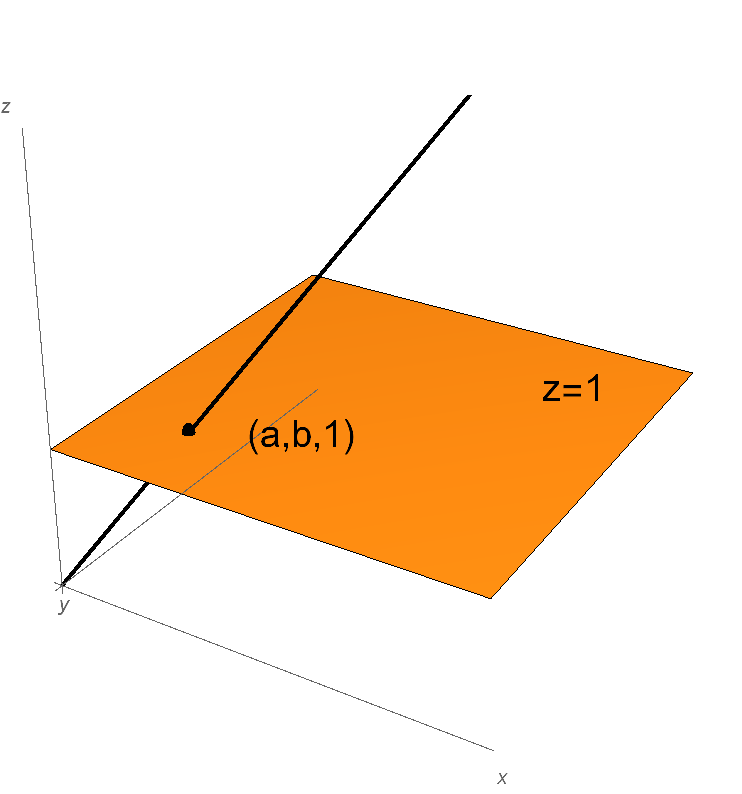
\includegraphics[width=0.5\textwidth]{images/projektivna_ravnina_mathematicafix.pdf}
\captionof{figure}{Projektivna ravnina}
\end{figure}
}

\frame{
\frametitle{Osnovni pojmi}
\begin{block}{Algebraična krivulja}
\emph{Algebraična krivulja}, podana s homogenim polinomom $P$, je množica točk 
$$\mathcal{C}_P= \{ A \in \mathbb{P}^2, P(A) = 0 \}.$$
\end{block}

\begin{block}{Kubična krivulja}
\emph{Kubična krivulja} je algebraična krivulja, podana s homogenim polinomom stopnje 3. V splošnem je polinom oblike
\begin{align}
&{} a_{300}x^3+a_{210}x^2y+a_{201}x^2z+a_{120}xy^2+a_{102}xz^2+ \nonumber \\
&{}+a_{012}yz^2+a_{030}y^3+a_{003}z^3+a_{111}xyz+a_{021}y^2z, \nonumber
\end{align}
kjer so $a_{ijk} \in \F$.
Ta zapis vsebuje $10$ koeficientov, vendar se lahko v gladkih primerih polinom poenostavi z ustrezno zamenjavo spremenljivk.
\end{block}

}

\frame{
\frametitle{Osnovni pojmi}
\begin{block}{Gladkost}
Algebraična krivulja je \emph{gladka}, če nima singularne točke.
\end{block}

\begin{block}{Izrek}
Enačbo gladke kubične krivulje nad algebraično zaprtim poljem lahko zapišemo v Weierstrassovi obliki
$$y^2z = x^3 + axz^2 + bz^3.$$
\end{block}
}

\frame{
\begin{figure}[ht]
\centering
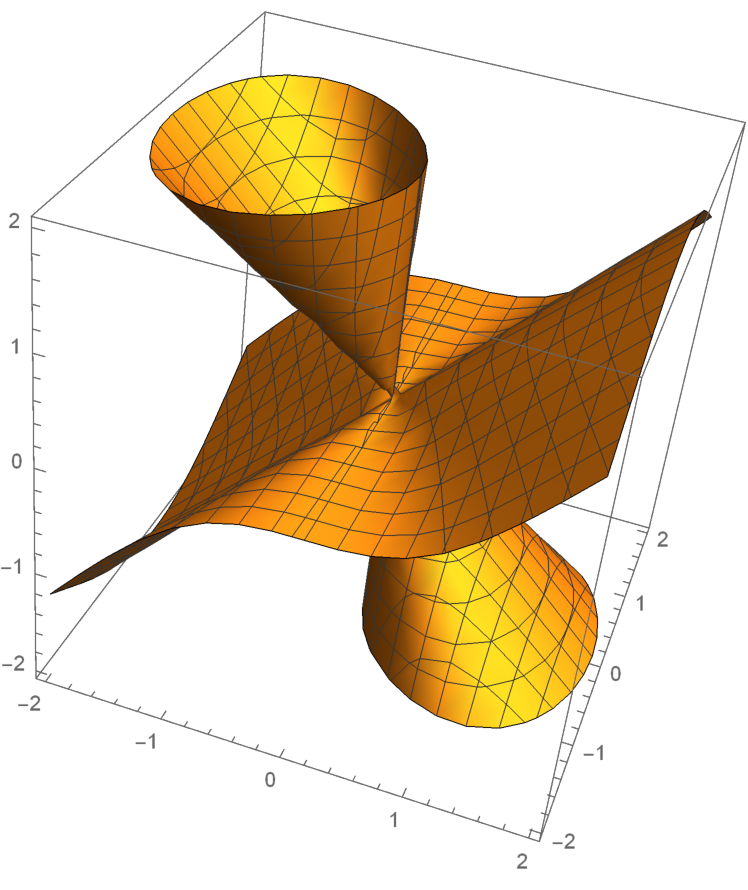
\includegraphics[width=0.5\textwidth]{images/krivulja_v_r3.pdf}
\captionof{figure}{$y^2z = x^3-xz^2$}
\end{figure}
}

\frame{
\frametitle{Zgled v projektivni ravnini $z=1$}

\begin{figure}[ht]
\centering
\begin{minipage}{.5\textwidth}
\centering
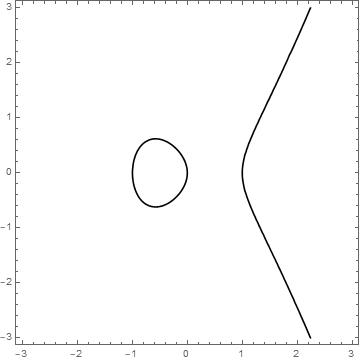
\includegraphics[scale=0.4]{images/slika1.jpg}
\captionof{figure}{$y^2 = x^3-x$}
\end{minipage}%
\begin{minipage}{.5\textwidth}
\centering
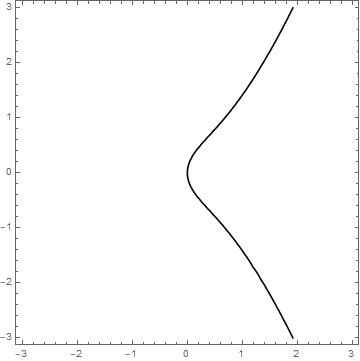
\includegraphics[scale=0.4]{images/slika2.jpg}
\captionof{figure}{$y^2=x^3+x$}
\end{minipage}
\end{figure}
}

\frame{
\frametitle{Grupa nad kubičnimi krivuljami}
Za definicijo grupe na kubičnih krivuljah nad $\C$ najprej uvedimo pomožno operacijo

$$\ast : \mathcal{C}_P \times \mathcal{C}_P \rightarrow \mathcal{C}_P,$$
tako da za poljubni točki $A$, $B$ na krivulji velja:

\[ A \ast B =
\begin{cases}
A & \quad \text{če je } A=B \ \text{prevoj},\\
C & \quad \text{če je } \overline{AB} \cap \mathcal{C}_P = \left\{ A,B,C \right\},\\
A & \quad \text{če je } \overline{AB} \ \text{tangenta v } A,\ \text{ter} \ A \neq B,\\
B & \quad \text{če je } \overline{AB} \ \text{tangenta v } B,\ \text{ter} \ A \neq B,\\
C &\quad \text{če je } A=B \  \text{in}\ \{\text{tangenta v A}\} \cap \mathcal{C}_P = \left\{ A,C \right\}.\\
\end{cases}
\]

}

\frame{
\frametitle{Grupa nad kubičnimi krivuljami}
\begin{izrek}
Kubična krivulja ($\mathcal{C}_P$,$+$) je Abelova grupa za operacijo

\begin{table}[ht]
\centering
\begin{tabular}{llll}
$+:$ & $\mathcal{C}_P \times \mathcal{C}_P$ & $\rightarrow$ & $\mathcal{C}_P$ \\
& $(A,B)$ & $\mapsto$ & $(A\ast B)\ast O$ ,
\end{tabular}
\end{table}
kjer je $O$ poljubna izbrana točka na krivulji $ \mathcal{C}_P$.
\end{izrek}
\begin{opomba}
Za kubično krivuljo v Weierstrassovi obliki za točko $O$ ponavadi izberemo tako imenovano točko v neskončnosti, oblike $[0,1,0]$, ki jo označimo z $\infty$.
\end{opomba}
}

\frame{
\frametitle{Grupa nad kubičnimi krivuljami}
\begin{figure}[ht]
\centering
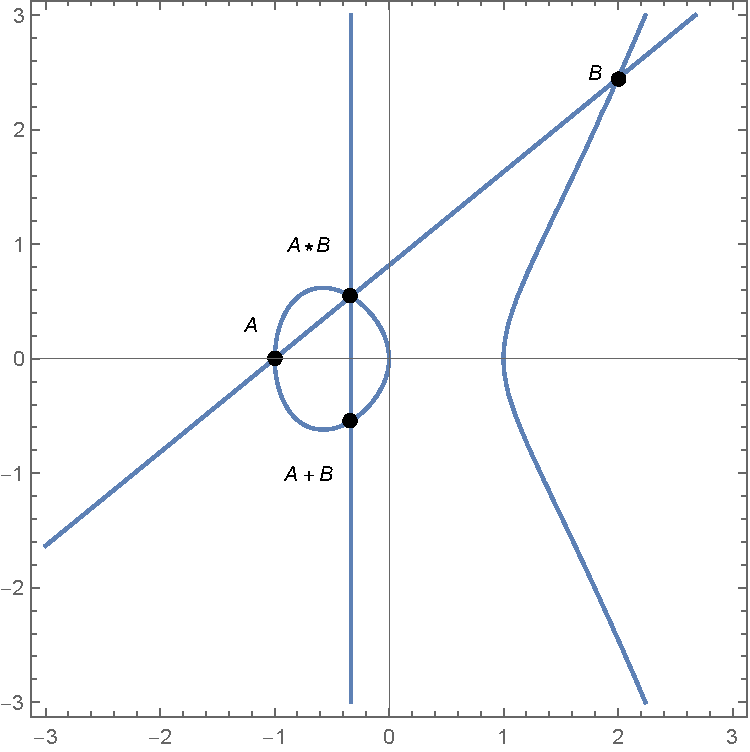
\includegraphics[width=0.5\textwidth]{images/sestevanje_tock_mathematicafix.pdf}
  \caption[Grafično seštevanje.]{Grafično seštevanje točk na kubični krivulji.}
\end{figure}

}
 

\frame{
\frametitle{Eliptične krivulje mod $p$}

Za dani števili $a$, $b \in \mathbb{Z}/p\mathbb{Z}$ je \emph{kubična krivulja} nad poljem $\mathbb{Z}/p\mathbb{Z}$ množica točk
$$E_{(a,b)}(\mathbb{Z}/p\mathbb{Z}) =\left\{ [x,y,z] \in \PP^2(\mathbb{Z}/p\mathbb{Z}): y^2z=x^3+axz^2+bz^3 \right\} .$$
Drugače povedano, afina kubična krivulja je množica rešitev Weierstrassove enačbe
$$y^2=x^3+ax+b,$$
pri čemer upoštevamo zvezo med afinimi in projektivnimi koordinatami točk:
$$(x,y)\in (\mathbb{Z} /p\mathbb{Z})^2 \Leftrightarrow [x,y,1]\in \PP^2(\mathbb{Z}/p\mathbb{Z} ).$$
%V nadaljevnaju bomo za polja uporabljali oznako $\F{q}$, ki predstavlja $\Z{p^k}$.
}

%zgled $y^2 = x^3+x+1$ nad $F_5$ kniga stran 95.



\frame{
\frametitle{Torzijske točke}
\begin{definicija}
Naj bo $E$ eliptična krivulja nad poljem $K$, ter naj bo $n\in \N$. \emph{Torizjske točke} reda $n$, so točke v množici
$$E[n] = \{ P \in \E{\overline{K}} | nP = \infty \}.$$
\end{definicija}


\begin{izrek}
\label{IzrekTor}
Naj bo $E$ eliptična krivulja nad poljem $K$ in naj bo $n \in \N$. Če karakteristika polja $K$ ne deli $n$ oziroma je enaka $0$, potem je
$$E[n] \cong \mathbb{Z}_n \oplus \mathbb{Z}_n.$$

Zapišimo $n=p^rn'$, kjer $p$ ne deli $n'$. Če je karakteristika $K$ enaka $p >0$ in $p|n$, potem velja
$$E[n] \cong \mathbb{Z}_{n'} \oplus \mathbb{Z}_{n'} \text{ ali } E[n] \cong \mathbb{Z}_n \oplus \mathbb{Z}_{n'}.$$

\end{izrek}


}


\frame{
\frametitle{Endomorfizem}
\begin{definicija}
Naj bo $K$ polje nad katerim je definirana eliptična krivulja $E$.
\emph{Endomorfizem} na $E$ je homomorfizem $\alpha: \E{\overline{K}} \rightarrow \E{\overline{K}} $, ki je podan z racionalno funkcijo. Torej obstajata racionalni funkciji $R_1$ in $R_2$ s koeficienti v $\overline{K}$ za kateri velja
$$\alpha(x,y) = (R_1(x,y),R_2(x,y)),$$
za vse $(x,y) \in \E{\overline{K}}$.
\end{definicija}

\begin{block}{Standardizirana oblika}
Endomorfizem $\alpha$ lahko zapišemo v standardizirani obliki
$$\alpha(x,y) = (r_1(x),r_2(x)y), \text{ kjer je} r_1(x) = \frac{p(x)}{q(x)}.$$
\end{block}
}

\frame{

\begin{definicija}
\emph{Stopnja} endomorfizma je  definirana kot
$$
\DEG{\alpha} =
\begin{cases}
\max \{ \deg{p(x)},\deg{q(x)} \} & \text{če }\alpha \not\equiv 0, \\
0 & \text{če } \alpha \equiv 0.
\end{cases}
$$
\end{definicija}

\begin{definicija}
Netrivialni endomorfizem $\alpha$ je \emph{separabilen}, če je odvod $r'_1(x) \not \equiv 0$.
\end{definicija}
}

\frame{
\frametitle{Frobeniusov endomorfizem}
Naj bo $\F_q$ končno polje z algebraičnim zaprtjem $\overline{\F_q}$ in naj bo
\begin{align}
\phi_q:\overline{\F_q} &{} \rightarrow \overline{\F_q}, \nonumber \\
x &{} \mapsto x^q \nonumber
\end{align}
Frobeniusova preslikava na $\F_q$.
Če je eliptična krivulja $E$ definirana nad $\F_q$, potem $\phi_q$ deluje na točkah $E$ kot:
$$\phi_q(x,y) = (x^q,y^q) \text{ in } \phi_q(\infty) = \infty.$$
}

\frame{
\frametitle{Hassejev izrek}

\begin{izrek}[Hasse]
\label{izr:Hasse}
Naj bo $E$ eliptična krivulja nad končnim poljem $\F_q$.  Potem red $\E{\F_q}$ zadošča zvezi
$$|q+1-\#\E{\F_q}| \leq 2\sqrt{q}.$$
\end{izrek}

}

\frame{
\frametitle{Red grupe}
\begin{trditev}
\label{trd:4.12}
Naj bo $\# \E{\F_q} = q+1-a$. Zapišimo $X^2-aX+q = (X-\alpha)(x-\beta)$. Potem velja
$$\# \E{\F_{q^{n}}} = q^n+1-(\alpha^n+\beta^n),$$
za vse $n \geq 1$.

\end{trditev}
}

\frame{
\frametitle{Delitelji}
\begin{block}{Delitelj}
Naj bo $K$ polje in naj bo $P$ točka na krivulji $\E{\overline{K}}$. Za vsako točko $P$ definirajmo formalen simbol $[P]$. \emph{Delitelj} $D$ na krivulji $E$ je končna linearna kombinacija takih simbolov s celoštevilskimi koeficienti
$$D = \sum_{j}a_j[P_j], \ a_j \in \Z.$$
\end{block}

\begin{block}{Definicija}
Definirajmo \emph{vsoto} in \emph{stopnjo} delitelja kot
$$\SUM{\sum_{j}a_j[P_j]} = \sum_ja_jP_j \ \in \E{\overline{K}},$$
$$\DEG{\sum_{j}a_j[P_j]} = \sum_ja_j \ \in \Z.$$
\end{block}
}

\frame{
\begin{definicija}
Naj bo $E$ eliptična krivulja nad poljem $K$. \emph{Funkcija} na $E$ je racionalna funkcija $$f(x,y) \in \ \overline{K},$$ ki je definirana za vsaj eno točko na $\E{\overline{K}}$. Funkcija torej zavzame vrednosti v $\overline{K}$.
\end{definicija}

\begin{trditev}
Naj bo $P$ točka na krivulji $E$. Potem obstaja funkcija $u_P$, kateri rečemo uniformizator, z lastnostjo $u_P(P) = 0$, za katero velja, da lahko vsako funkcijo $f(x,y)$ nad $E$ zapišemo kot
$$f = u^r_Pg, \text{ za nek } r\in \Z, \text{ kjer } g(P) \neq 0 \text{ in } \frac{1}{g(P)} \neq 0.$$
\end{trditev}
}

\frame{
\begin{definicija}
Številu $r$ iz trditve  rečemo \emph{red} funkcije $f$ v točki $P$ in ga označimo z $\ORDp{f}{P}$.
\end{definicija}

\begin{definicija}
Naj bo $f$ funkcija nad $E$, ki ni identično enaka $0$. Definirajmo \emph{delitelj} funkcije $f$ kot
$$\Div{f} = \sum_{P\in \E{\overline{K}}} \ORDp{f}{P}[P] \in \DIV{E}.$$
\end{definicija}
}

\frame{
\frametitle{Weilovo parjenje}

\begin{definicija}
Naj bo $K$ polje in naj bo $n \in \N$ tak, da karakteristika $K$ ne deli $n$.
$$\mu_n = \{ x \in \overline{K} | x^n = 1 \}$$
je \emph{grupa n-tih korenov enote} $\overline{K}$.
\end{definicija}

}


\frame{
\frametitle{Weilovo parjenje}

\begin{izrek}
Naj bo E eliptična krivulja definirana nad poljem $K$, in naj bo $n \in \N$. Predpostavimo, da karakteristika polja $K$ ne deli $n$. Potem obstaja Weilovo parjenje
$$e_n:E[n] \times E[n] \rightarrow \mu_n,$$
za katerega velja:
\begin{itemize}
\item $e_n$ je bilinearna v obeh spremenljivkah
$$e_n(S_1+S_2,T) = e_n(S_1,T)e_n(S_2,T)$$
in
$$e_n(S,T_1+T_2) = e_n(S,T_1)e_n(S,T_2)$$
za vse $S,S_1,S_2,T,T_1,T_2 \in E[n]$.
\end{itemize}
\end{izrek}

}

\frame{
\begin{izrek}[nadaljevanje]
\begin{itemize}

\item $e_n$ je neizrojena v obeh spremenljivkah. To pomeni, $e_n(S,T) = 1$ za vse $T \in E[n]$ natanko tedaj, ko je $S = \infty$.

\item $e_n(T,T) = 1$ za vse $T \in E[n]$.

\item $e_n(T,S) = e_n(S,T)^{-1}$ za vse $S,T \in E[n]$.

\item $e_n(\rho S,\rho T) = \rho(e_n(S,T))$ za vse avtomorfizme $\rho$ na $\bar{K}$, za katere je $\rho$ identiteta na koeficientih enačbe za $E$.

\item $e_n(\alpha(S),\alpha(T)) = e_n(S,T)^{\DEG{\alpha}}$ za vse separabilne endomorfizme $\alpha$ polja $E$.



\end{itemize}
\end{izrek}
}

\frame{
\frametitle{Millerjev algoritem}
\begin{izrek}
\label{izrek:Miller}
Naj bo $E$ eliptična krivulja in naj bosta $P=(x_P,y_P), Q = (x_Q,y_Q)$ ne ničelni točki na $E$.
\begin{enumerate}
\item Označimo z $\lambda$ naklon premice, ki povezuje točki $P,Q$. V primeru, da sta ti točki enaki, $\lambda$ predstavlja naklon tangente v točki. Če je premica navpična ($x_P = x_Q$), potem privzamemo, da je $\lambda = \infty$. Definirajmo funkcijo $g_{P,Q}$ na sledeči način:
\[ g_{P,Q} =
\begin{cases}
\frac{y-y_P-\lambda(x-x_P)}{x+x_P+x_Q-\lambda^2} & \quad \text{če } \lambda \neq \infty ,\\
x-x_P & \quad \text{sicer} .\\
\end{cases}
\]

Potem velja 
$$\Div{g_{P,Q}} = [P] + [Q] - [P+Q] - [\infty].$$



\end{enumerate}


\end{izrek}

}

\frame{

\begin{izrek}[nadaljevanje]
\begin{enumerate}
\item (Millerjev algoritem) Naj bo $m \geq 1$. Zapišimo $m$ v binarnem kot
$$m = m_0+m_1\cdot 2 + m_2\cdot 2^2 + \ldots + m_{n-1}\cdot 2^{n-1},$$
kjer so $m_i \in \{ 0,1 \}$ in $m_{n-1} \neq 0$. Potem algoritem~\ref{alg:Miller} vrne
funkcijo $f_P$, za katero velja
$$\Div{f_P} = m[P]-[mP]-(m-1)[\infty].$$ 
\end{enumerate}
\end{izrek}

}

\begin{frame}[fragile]

\begin{algorithm}[H]
\caption[Miller]{Millerjev algoritem}
\label{alg:Miller}

\begin{algorithmic}[1]
\State Vhod: število m podano v binarnem zapisu, točka P na eliptični krivulji
\State Izhod: funkcija $f_P$
\State $T = P,f = 1$
\For {$i = n-2:0$}
	\State $f = f^2 \cdot g_{T,T}$
	\State $T = 2T$
	\If {$m_i = 1$}
		\State $f = f \cdot g_{T,P}$
		\State $T=T+P$
	\EndIf
	
\EndFor

\end{algorithmic}
\end{algorithm}

\end{frame}

\frame{
\frametitle{Diffie-Hellmanova izmenjava ključev nad eliptičnimi krivuljami}

\begin{enumerate}

\item Alenka in Boris se dogovorita za eliptično krivuljo $E$ nad končnim obsegom $\Fq{q}$, ter za točko $P \in \E{\Fq{q}}$.
\item Alenka se naključno odloči za skrivno število $a \in \N$, in izračuna $P_a = aP$, ter to pošlje Borisu. Pri tem red točke $P$ ne sme biti enak $a$.
\item Boris se naključno odloči za skrivno število $b \in \N$, in izračuna $P_b = bP$, ter to pošlje Alenki. Pri tem red točke $P$ ne sme biti enak $b$.
\item Alenka izračuna $aP_b=abP$.
\item Boris izračuna $bP_a=baP$.
\item Skupni ključ je $abP$.

\end{enumerate}

}

%Edine informcije, ki jo tako dobi nek prisluškovalec so krivulja $E$, končni obseg $\Fq$, ter točke $P, aP,bP$. Iz tega pa mora izračunati $abP$.

\frame{
\frametitle{Problem diskretnega logaritma}
\begin{definicija}
Naj bo $G$ grupa, kjer njeno operacijo označimo z $\circ$.
Naj bosta $a, b \in G$. Naj $b^k$ označuje $$b^k = \underbrace{b\circ b\circ \cdots \circ b}_\text{$k$-krat}.$$ Število $k \in \N$, ki reši enačbo $$b^k = a$$ imenujemo \emph{diskretni logaritem} elementa $a$ pri osnovi $b$.

\end{definicija}

}

\frame{
\frametitle{Problem diskretnega logaritma}
Problem Diffie-Hellmanove izmenjave ključev lahko prevedemo na problem diskretnega logaritma na sledeč način
\begin{itemize}
\item Vzemi $aP$ in izračunaj $a$ tako, da rešiš problem diskretnega logaritma.
\item Izračunaj $a(bP)$.
\end{itemize}

Velja torej:
$$\text{DL} \Rightarrow DH$$

}

%Če Eva lahko reši problem diskretnega logaritma v $\E{\Fq}$, potem lahko iz $P$ in $aP$ izračuna $a$ ter nato izračuna $abP$, ter na ta način dobi ključ.

\frame{
\frametitle{MOV napad}
MOV napad uporabi Weilovo parjenje, da pretvori problem diskretnega logaritma iz $E(\Fq{q})$ v problem diskretnega logaritma nad $\Fq{q^m}^x$. Nato pa diskretni logaritem nad novim poljem napademo s pomočjo algoritma izračun indeksa. To deluje če velikost polja $\Fq{q^m}$ ni dosti večja od velikosti polja $\Fq{q}$. Postopek napada sledi poteku dokaza naslednje trditve.

\begin{trditev}
Naj bo $E$ eliptična krivulja nad $\Fq{q}$. Naj bosta $P,Q \in E(\Fq{q})$, ter naj bo $N$ red točke $P$. Predpostavimo, da velja $\text{gcd}(N,q)=1$. Potem obstaja tako število $k$, da velja $Q = kP$ natanko tedaj ko $NQ = \infty$ in $e_N(P,Q)=1$.
\end{trditev}

}

\frame{
\frametitle{MOV napad}

Izberi $m$ tako, da $$E[N] \subset \E{\Fq{q^m}}.$$

Ker imajo vse točke $E[N]$ koordiante v $\overline{\Fq{q}} = \cup_{j\geq 1}\Fq{q^j}$ tak $m$ obstaja. Prav tako je $\mu_N$ v $\Fq{q^m}$.

\begin{enumerate}
\item Izberi točko $T \in \E{\Fq{q^m}}$.
\item Izračunaj red $M$ točke $T$.
\item Naj bo $d = \text{gcd}(M,N)$ in naj bo $T_1 = (M/d)T$. Potem ima $T_1$ red, ki deli $N$, torej je $T_1 \in E[N]$.
\item Izračunaj $\zeta_1 = e_N(P,T_1)$ in $\zeta_2 = e_N(Q,T_1)$. Tu sta $\zeta_1$ in $\zeta_2$ v $\mu_d \subset \Fq{q^m}^\times$.
\item Reši problem diskretnega logaritma $\zeta_2 = \zeta_1^k$ v $\Fq{q^m}^\times$. To nam da $k \mod d$.
\item Ponovi za različne točke $T$ dokler ni $k$ določen.
\end{enumerate}


}

\frame{
\frametitle{Anomalne krivulje}
\begin{definicija}
Krivulji $E$ nad poljem $\F_q$, za katero velja
$$\#\E{\F_q} = q,$$
rečemo \emph{anomalna krivulja}.

\end{definicija}

\begin{trditev}
\label{trd:5.6}
Naj bo $E$ eliptična krivulja nad $\F_p$ in naj bosta $P,Q \in \E{\F_p}$. Predpostavimo še, da je krivulja $E$ oblike $y^2=x^3+ax+b$. Potem obstajajo cela števila
$a',b',x_1,x_2,y_1,y_2$ in eliptična krivulja $E'$ podana z
$$y^2=x^3+a'x+b',$$
ter točke $P'=(x_1,y_1),Q'=(x_2,y_2), \in E'(\Q)$.
Za ta števila velja
$$a\equiv a',\ b \equiv b',\ P \equiv P',\ Q \equiv Q' \MOD{p}.$$

\end{trditev}

}

\begin{frame}[fragile]
\begin{algorithm}[H]
\caption[ANC]{Napad na anomalne krivulje}
\label{alg:AnomalAttack}
Vhod: Točki $P, Q$ nad eliptično krivuljo $E$.\newline
Izhod: diskretni logaritem $k$.\newline
\begin{enumerate}
\item Razširi $E,P,Q$ nad $\mathbb{Z}$, kot v trditvi~\ref{trd:5.6}.
\item Izračunaj $P_2' = (p-1)P' \equiv (x',y') \MOD{p^2}$.
\item Izračunaj $Q_2' = (p-1)Q' \equiv(x'',y'') \MOD{p^2}$.
\item Izračunaj
$$m_1 = p\frac{y'-y_1}{x'-x_1}, \ m_2 = p\frac{y''-y2}{x''-x_2}.$$
\item Če $v_p(m_2) <0$ ali $v_p(m_1)<0$ poizkusi na drugi krivulji $E'$. V nasprotnem primeru je $k \equiv m_1/m_2 \MOD{p}$.
\end{enumerate}

\end{algorithm}
\end{frame}




\end{document}
